\subsection{Anwendung und Test}
Um die Implementierungen der Schnittstellen zur ArangoDB zu testen, werden die beiden Webservices (Java und FOXX) abgefragt. Das Frontend kann unter folgendem Link im Cluster erreicht werden: \texttt{http://10.20.110.61/team38/sdb-foxx-service/} \newline
Um zufällige Schwankungen abzufangen, werden bei jeden Szenario mehrere Requests gemacht und ein Durchschnittswert ermittelt. Die Tests der Anwendungsszenarien werden mit jeweils 100 Anfragen getestet. Daraus ergeben sich dann folgende Ergebnisse:
\begin{figure}[htbp] 
  	\centering
     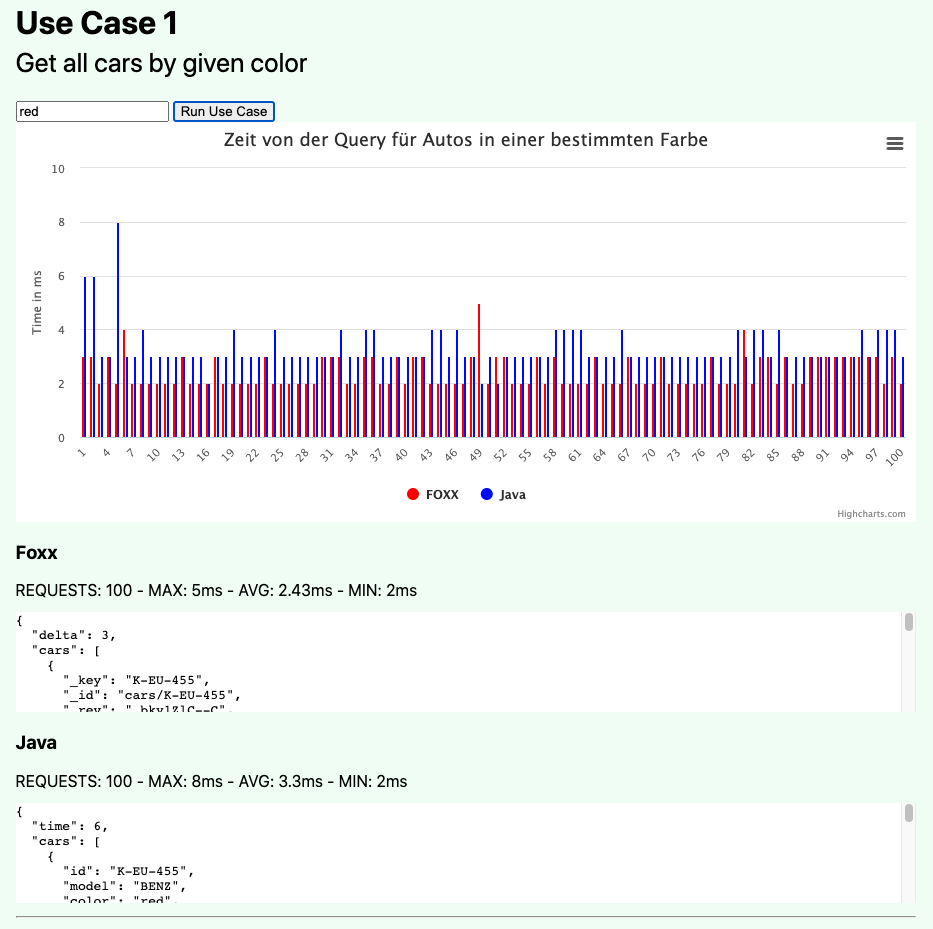
\includegraphics[width=1\textwidth]{./images/UseCase1.png}
 	\caption{Anwendungsszenario 1 Ergebnisse}
  \label{fig:DataSchema}
\end{figure}
\begin{figure}[htbp] 
  	\centering
     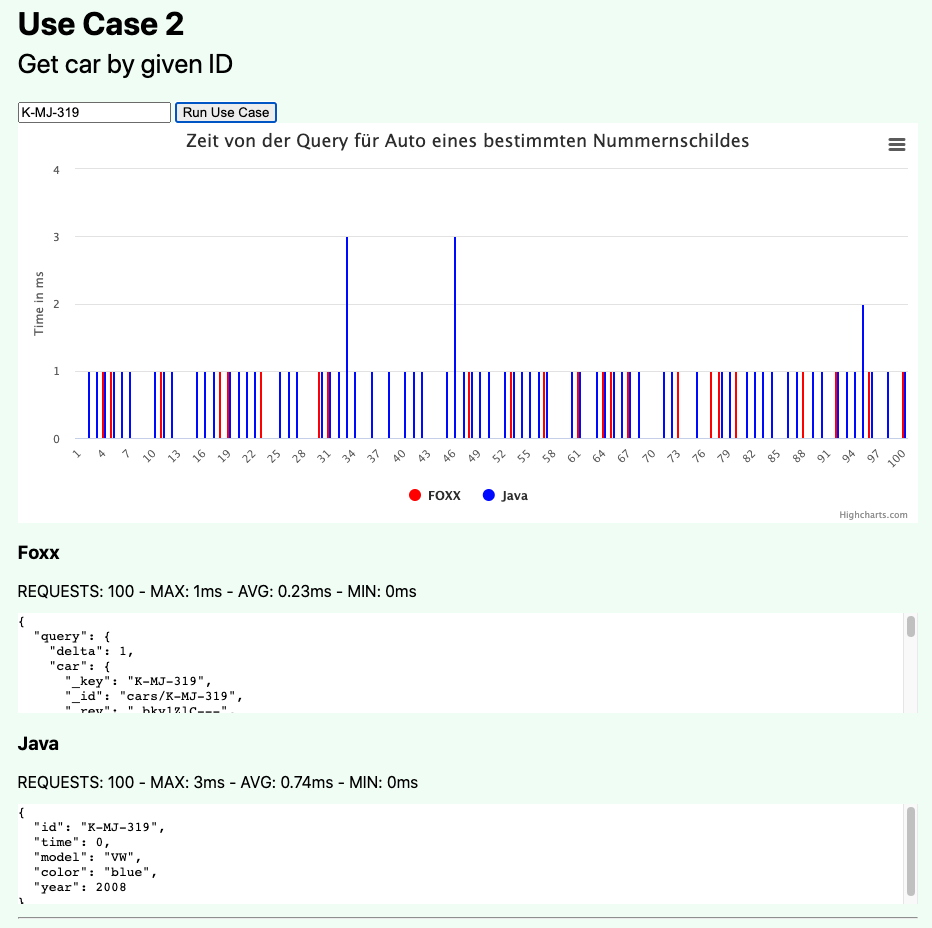
\includegraphics[width=1\textwidth]{./images/UseCase2.png}
 	\caption{Anwendungsszenario 2 Ergebnisse}
  \label{fig:DataSchema}
\end{figure}
\begin{figure}[htbp] 
  	\centering
     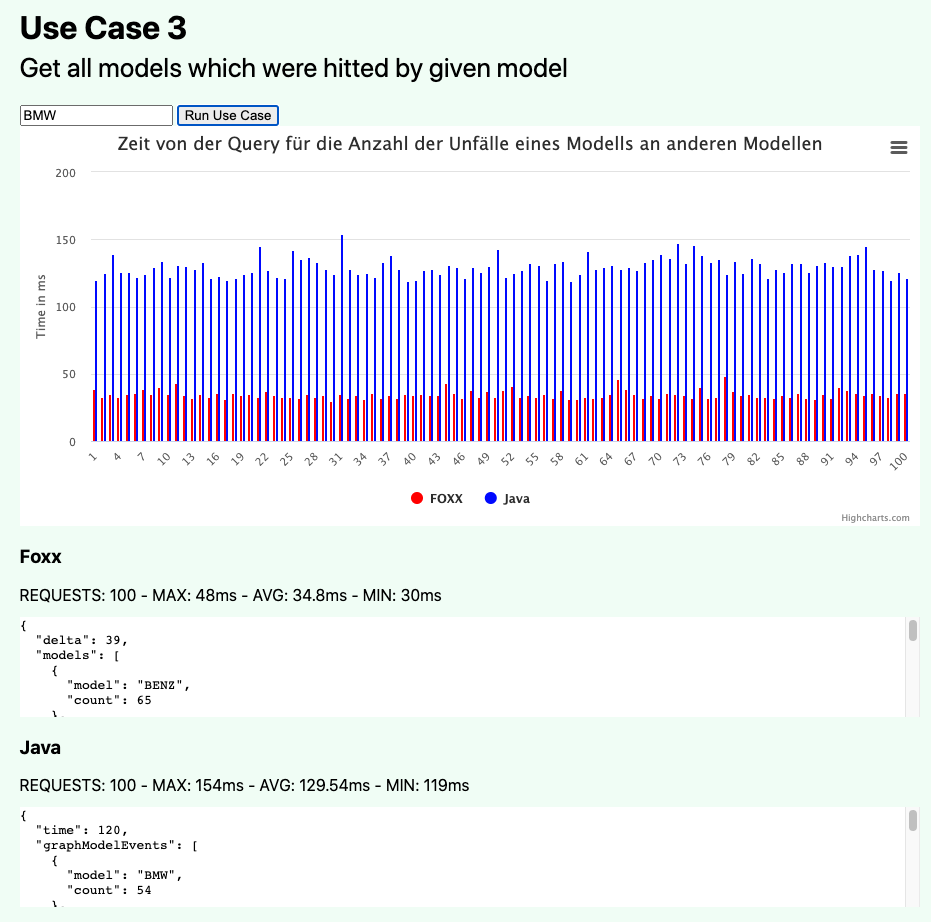
\includegraphics[width=1\textwidth]{./images/UseCase3.png}
 	\caption{Anwendungsszenario 3 Ergebnisse}
  \label{fig:DataSchema}
\end{figure}